
\section{Empirical Behavior of the Proposed Method
}
\label{sec:empirical-evaluation}

In this section we examine the behaviour of our method when confronted with certain isolated difficulties. 
Instead of relying on a computed approximation $\hat{\rho}_\delta$, we assume we are given the actual perturbed density $\rho_\delta$ explicitly or we compute it through numerical integration. This ensures that any error observed during this analysis is caused directly by our LIDL method and not the density estimator. However, it comes at a price of restricting us to relatively simple examples where we can efficiently compute $\rho_\delta$. 


\subsection{Uniform density on an interval}

\begin{figure}[t]
    \centering
    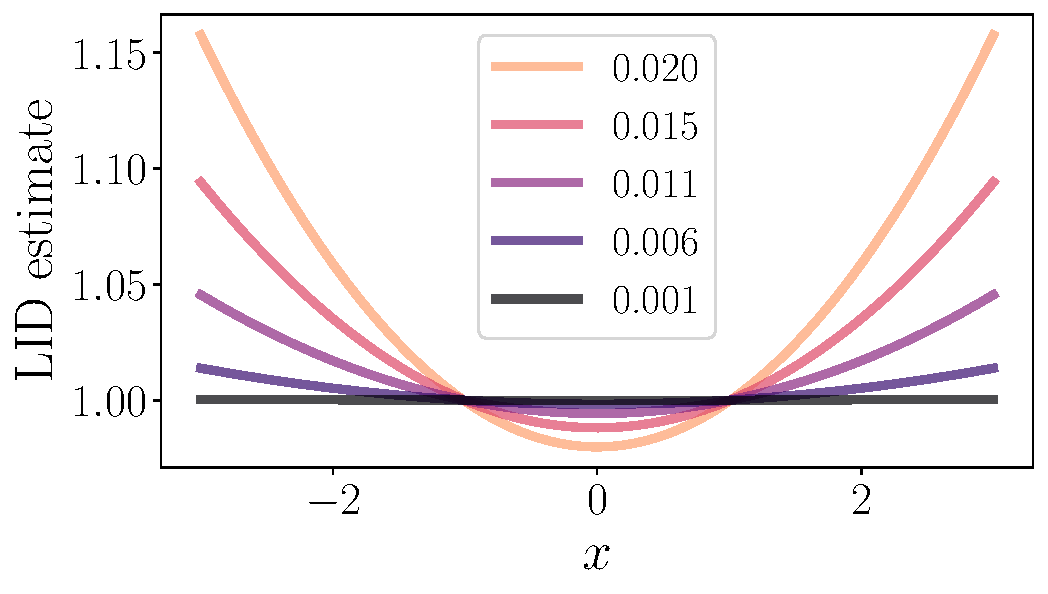
\includegraphics[width=0.4\textwidth]{images/evaluation-normal.pdf}
    \caption{LIDL estimates for points from $\N(0,1)$ for different values of $\delta$ marked with different colors, as explained in the legend of the plot.}
    \label{fig:evaluation-normal}
\end{figure}

We assume, that in the neighborhood of $x$ the density is bounded from below by a positive constant. But for some real-world cases, this assumption is not fulfilled. To investigate how LIDL behaves in this case we ran it on $\U(0,1)$. It can be seen as a distribution on the real line, whose density vanishes outside $[0,1]$ interval, violating this assumption. Alternatively, in the vicinity of the interval endpoints, the size of the neighborhood admitting the parametrization required for the proof of the core estimate decreases to $0$.

We analytically calculated the convolution of $\U(0,1)$ with $\N(0,\delta^2)$ and used it to estimate LID at 1000 points between 0 and 1. 
We used just two points for linear regression, corresponding to $\delta_1=\delta$ and $\delta_2=1.05\delta$. The estimates for different values of $\delta$ are plotted in Fig.~\ref{fig:evaluation-uniform}. We can see that an error is introduced near the boundary as expected. In this case, its maximum value does not depend on the value of $\delta$, and points affected by this problem lie in the part closer than $\sim4\delta$ to the endpoints of the distribution support.


\subsection{Normal distribution on a line}


In this example, we study the LID estimates at different points of a line embedded in $\R^D$.
In Fig.~\ref{fig:evaluation-normal} we can see the estimates computed as per the previous example, for a few values of $\delta$. 
At first glance, it is worrying that the error seems to explode with distance from the mean of the distribution.
In Appendix~\ref{sec:appendix-lidl-for-normal-distribution}, we show that the error is quadratic in this distance, and, reassuringly, that its expected value over the whole distribution can be controlled.
The reason for this behavior can be traced back to the proof of Lemma~\ref{lem:tangent-gaussian-estimate} (more specifically eq.~\eqref{eq:approximating-integral-of-tangential-normal-distribution} in the appendix), which depends on the positive constant locally bounding the density from below. 
In our example, the density decreases as $e^{-t^2/2}$, which produces the quadratic error term (the final error is bounded by $\sum_i\abs{\log C_i}$, where $C_i$ are the multiplicative estimate constants appearing in all the steps of the proof). 

\subsection{Uniform density on a curved manifold}

\begin{figure}[tb]
    \centering
    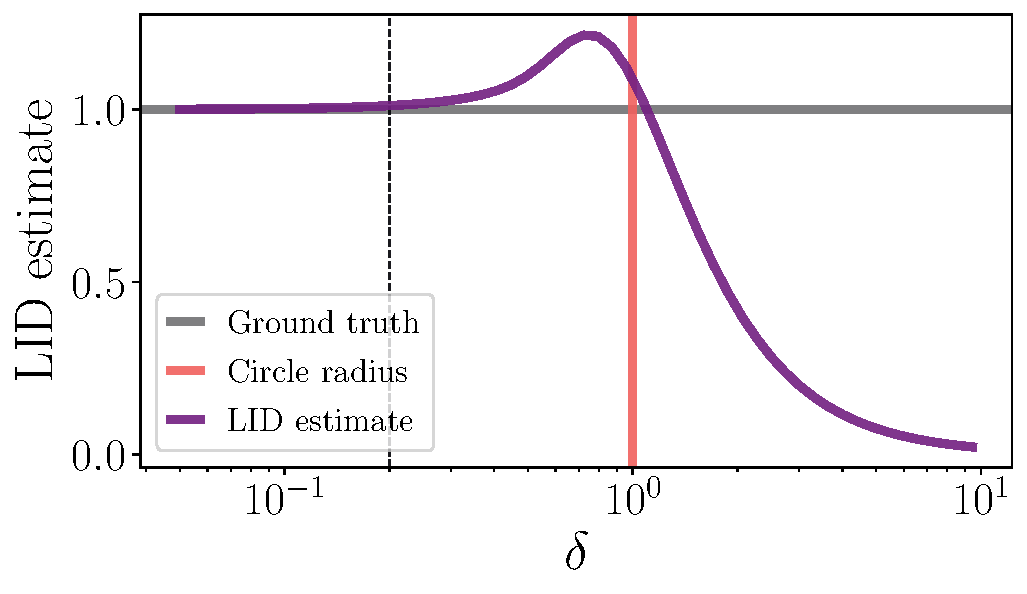
\includegraphics[width=0.4\textwidth]{images/evaluation-curvature.pdf}
    \caption{LIDL estimate as a function of $\delta$ for a uniform density on a unit circle. Vertical line at $\delta=0.2$.}
    \label{fig:evaluation-curvature}
\end{figure}


The LIDL estimate is affected by the curvature of the manifold, which manifests in the constant $C$ appearing in eq.~\eqref{eq:local-parametrization-norm-estimate}, subsequently used in the proofs of Lemmas~\ref{lem:ball-containment} and~\ref{lem:normal-gaussian-estimate}.
To see empirically how  the curvature influences the LIDL estimate, we numerically computed the convolution of the uniform density on the unit circle embedded in $\R^2$ with the noise distribution $\N(0,\delta^2I)$ for 2 values of $\delta$ similarly as in the previous examples. We calculated LIDL for the range of $\delta \in (0.05, 10)$. 
We plot the estimate dependence on $\delta$ in Fig.~\ref{fig:evaluation-curvature}. 

We can see that for $\delta \lesssim 0.2$ the estimate error is relatively small. After the positive bias for $\delta < 1$  we can observe a monotonic drop in the estimate until it reaches nearly 0. This is by the effect described in Section~\ref{sec:scale} where LIDL was observed to ignore the directions in which the standard deviations were lower than $\delta$.

\subsection{Manifolds with neighboring components}


In a real-world setting, it is possible for some connected components of the data manifold $S$ to be close to each other in the observable data space $\R^D$, especially when some features in the dataset have discrete distribution (e.g.\ height and sex in a medical dataset). In those settings, for values of $\delta$ comparable to the distance between the components, additional bias may be introduced to the estimate. To investigate this we ran an experiment similar to the previous example, but with a uniform distribution supported on the union of two long parallel segments. We then calculated LIDL estimates for the midpoints of those segments, to minimize the error caused by proximity to the boundary. We present the results in Fig.~\ref{fig:evaluation-close}. We can see positive bias in LIDL estimate appearing as $\delta$ is close to the distance between the segments, while for $\delta$ much larger than this distance, LIDL seems to view those two segments as a single line.

\subsection{Impact of linear regression on LIDL estimate}
Because our estimate depends on linear regression algorithm in order to estimate $\beta$, it may suffer from the same issues as any regression coefficient estimation algorithm \cite{li1985robust}, so in the future, more robust algorithm for linear regression estimation may be considered. Because we estimate only the rate of change, and not the constant from linear regression equation, LIDL is prone to biased log-likelihood estimates, and noise added to log-likelihood estimate only affects the variance of the estimate.

\begin{figure}[tb]
    \centering
    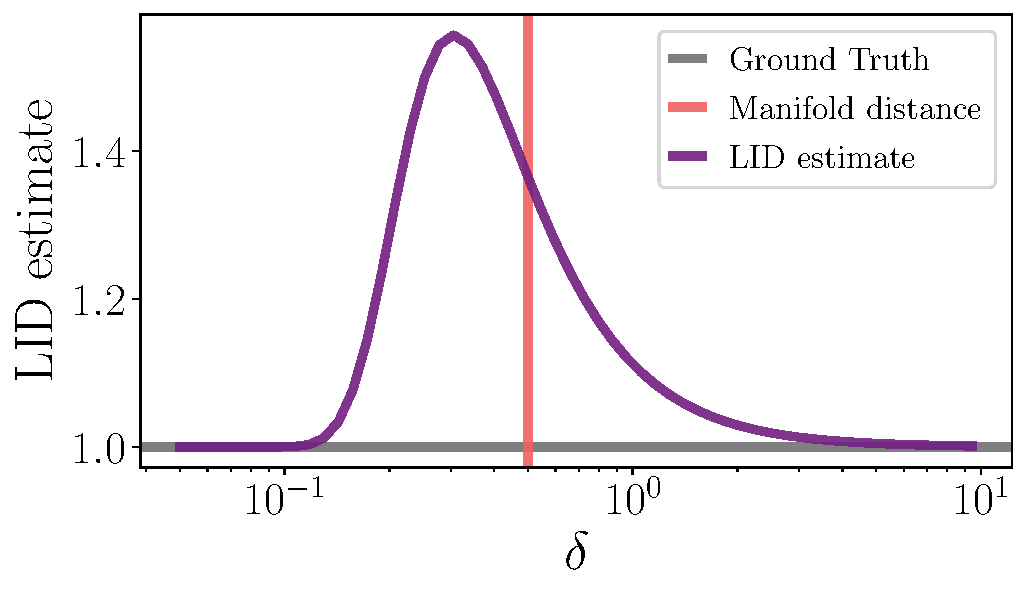
\includegraphics[width=0.4\textwidth]{images/evaluation-close.pdf}
    \caption{LIDL estimate as a function of $\delta$ for 2 long 1-dimensional manifolds parallel to each other.}
    \label{fig:evaluation-close}
\end{figure}


\subsection{Synthetic datasets}
\label{sec:other-perfect-datasets}
We ran evaluations of LIDL with density estimates computed using numerical integration on Swiss roll, uniform distribution on a helix, and Gaussians from 10 up to 4000 dimensions. We got almost exact estimates with mean absolute error (MAE) lower than $10^{-4}$ for every dataset. More information about these results is included in Appendix~\ref{sec:exp-details}.
